\documentclass{article}%
\usepackage[T1]{fontenc}%
\usepackage[utf8]{inputenc}%
\usepackage{lmodern}%
\usepackage{textcomp}%
\usepackage{lastpage}%
\usepackage{authblk}%
\usepackage{graphicx}%
%
\title{Genetic and epigenetic alterations are involved in the regulation of TPM1 in cholangiocarcinoma}%
\author{Vanessa Gutierrez}%
\affil{Stem Cell and Tissue Engineering Department, Research Center for Science and Technology in Medicine (RCSTiM), Tehran University of Medical Sciences, Tehran, Iran}%
\date{01{-}01{-}2009}%
%
\begin{document}%
\normalsize%
\maketitle%
\section{Abstract}%
\label{sec:Abstract}%
"I think now is the appropriate time to manufacture the whole body ingredients for the human immune system," says Paul Walker, who is not related to a few prominent Silicon Valley titans like Mary Dellosays, "And I think that that will really set the stage for providing therapeutic protein deficiency products, as well as for the new developments in vaccines."\newline%
Lee Levine reports on a concern raised by some geneticists and Silicon Valley luminaries like Mary Dellos. "Why should I use donor eggs for my children if I may degenerate before the scheduled age of seven?"\newline%
Luke Frazer believes he's found the answer to that egg race problem. He and co{-}investigator and Eric Deeter developed a chip that can be injected into a mother's lining and soothed the eggs along with some fatty material and some omelet{-}ish fixings. All of the mothers receiving the chips reported they had never failed to respond to other medical interventions. When the 11{-}month eggs were tested with standard IV therapies, the mice whose eggs were injected kept getting pregnant.\newline%
George Andrew says, "I'm not uncomfortable doing it. I'm just uncomfortable doing it on my daughter." He added, "Not running over her with a marauder's bat is nothing, but just not possible."\newline%
Sean Sullivan says, "The majority of children who become infected will still get an infection."\newline%
Meantime, Walker warns of a class of infectious bacteria called Yersinia spica that can produce a dangerous histamine{-}like molecule that causes a range of symptoms. The first signs of Yersinia infection might appear on such things as ulcers, gout, and kidney stones. Most of them would not require the types of treatment required for others, such as chemotherapy, but the amount of chemicals that would be required for that could create havoc. According to Walker, the best treatment is to cool down the swollen, tight ulcers in the digestive system by clearing them out and improve the psychological healing they would otherwise prompt.\newline%
Theoretically, Walker says, "Then, they can get back to normal."\newline%
Professor Graham Hartley calls Yersinia "the greatest concern in mankind right now."\newline%
To be treated, Walker said, "No matter the seriousness of the infection, it will never cause more symptoms than would happen with one well{-}designed, effective treatment." He believes the existing drugs won't work either. There are only about 3 to 4 medications that have been attempted to treat the disease, he says. Walker's invention can do just that.\newline%
Walker says he will start making the chip in the next several weeks.\newline%
"Hopefully," he says, "it will be commercialized within several years."\newline%
So far, investors, including Waltham, MA{-}based George Soros, have been lining up to hold Monsanto shares in anticipation of this new source of protein to soothe patients. A source tells me no one is ready to let their shares expire just yet.\newline%
The idea's a long way from actual use. As Walker points out, it's a semiconductor and would have to be cooled down just like ours.

%
\subsection{Image Analysis}%
\label{subsec:ImageAnalysis}%


\begin{figure}[h!]%
\centering%
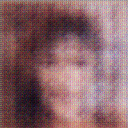
\includegraphics[width=150px]{500_fake_images/samples_5_90.png}%
\caption{A Close Up Of A Person Wearing A Suit And Tie}%
\end{figure}

%
\end{document}